%!TEX root = ../Thesis.tex
\chapter{Performance Assessment \& Verification of Aggregator Services} % (fold)
\label{cha:verification}
\newchapter{P}{erformance assessment is the} process\marginnote{The IEEE defines verification as:``confirmation, through the provision of objective evidence, that specified requirements have been fulfilled.''} of quantifying and verifying the provision of a service according to the contractual specifications of the service. Performance assessment usually occurs at three stages\fcite{coalition2014mapping}
\begin{itemize}
	\item To qualify potential resources against service specifications as part of the validation/prequalification procedure.
	\item To verify service conformance to the service specifications during and after service delivery. 
	\item To calculate the amount of service delivered by the resource as part of financial settlements.
\end{itemize}
%\begin{itemize}
%	\item Why is verification an important part of validation?
%	\item Performance Assessment of Aggregators providing Demand Response
%\end{itemize}
%All resources should be held to the performance specifications established by the product. However – demand side and generation side communication requirements will usually need to be designed separately and made appropriate to each. Technical rules often proscribe the use of metered values to base performance and settlements.[from the SEDC report used in the DRAS paper]

This chapter presents a novel set of performance indices developed for aggregator performance assessment, and how these can be used as part of aggregator validation and service verification. The initial work on aggregator performance assessment was presented in a conference paper\fcite{bondy2014performance} and further refined in a submitted journal paper\fcite{bondy2016method}. These paper can be found in Appendix~\ref{app:isgt2014} and Appendix~\ref{app:segan}. 
\section{Background}
\newsection{L}{ittle attention has been} given to the problem of performance assessment of aggregator controllers seen from a service-delivery perspective. As stated in Section~\ref{subsec:aggtest}, performance assessment of aggregators has been mostly ad-hoc analysis specific to a problem the designers are trying to solve, but none have taken a systematic approach to the evaluation of aggregators in terms of established service requirements.

Control Performance Assessment (CPA) is already an established field within control engineering. Most of the applications within the field are found in the process industry\ref{jelali2006overview}, but since aggregators are a control system, and provide control services, it is natural to translate concepts of CPA to the power system. Usually, CPA methods fall within two types:
\begin{itemize}
	\item benchmarking of controllers towards a theoretic optimum, taking stochasticity of the process into account; and
	\item benchmarking against deterministic properties required of the close-loop system.
\end{itemize}

Usually these indices are normed so that for an index $\eta$:
\begin{equation}
	\eta \in [0,1].
\end{equation}

\section{Quality of Service}\label{sec:MAINQoS}
\newsection{T}{he concept of Quality}\marginnote{This section relies heavily on the service modeling concepts presented in Chapter~\ref{cha:services}, and it is recommended that the reader familiarizes with that section before reading this section.} of Service (QoS) is closely related to the service models presented in Section\bondy{put in correct section reference}. One of the elements of a service model is the definition of the service error. QoS is an instantaneous measure of how well the aggregator is delivering a service at any given time instant, and can be defined as the scaling of the error to the limits defined in the service model, i.e.:
\begin{equation}
	QoS(t) = e(t)C_s(t),
\end{equation}
where $e(t)$ is the error in service delivery and $C_s(t)$ is a time varying normalization factor. This factor ensures that:
\begin{itemize}
	\item $QoS \geq 0$,
	\item for $QoS \leq 1$ the service is considered delivered within the contractual constraints, and
	\item $QoS = 0$ is a perfect service delivery.
\end{itemize}

The original definition proposed in \cite{bondy2014performance} assumed symmetric constraints around the acceptable provision, but in \cite{bondy2016method} this definition was expanded to account for asymmetry, thus $C_s(t)$ is defined as:
\begin{equation}
C_{s}(t) = 
\begin{cases}
\frac{1}{x_{acc,max}(t) - x_{max}(t)}, & e(t) \geq 0 \\
\frac{1}{x_{acc,min}(t) - x_{min}(t)}, & e(t) < 0.
\end{cases}\label{eq:MAINcst}
\end{equation}
where $x_{acc,max/min}$ and $x_{max/min}$ are part of the service model defined in Section~\bondy{refer to correct section}. A visual representation of the error models and their corresponding \emph{QoS} definition are shown in Figure~\ref{fig:MAINerrorQoS}

\begin{figure}[htpb!]
\centering
\subfloat[Tracking service error]{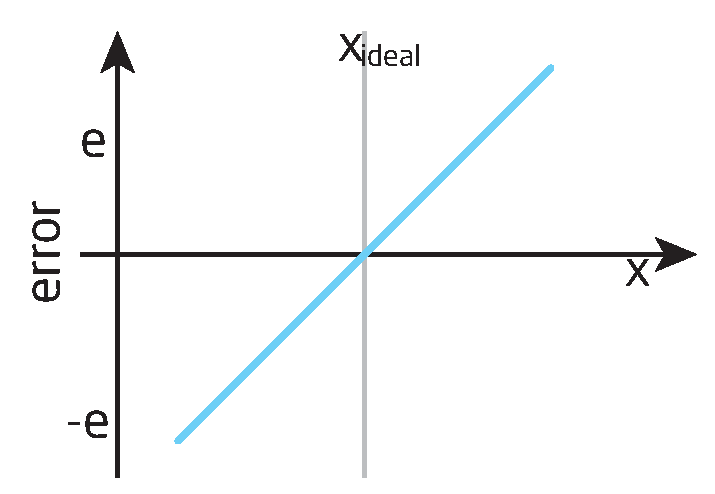
\includegraphics[width=0.5\columnwidth]{SEGAN/tracking_error2.eps}%
\label{subfig:errortracking}} \subfloat[Tracking service Quality of Service]{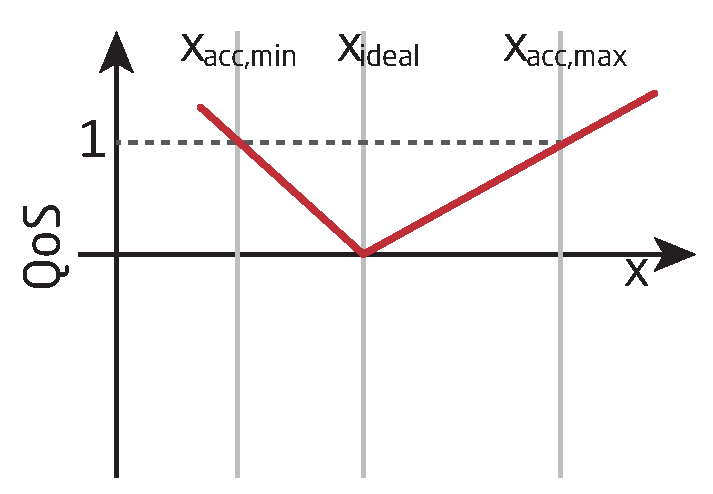
\includegraphics[width=0.5\columnwidth]{SEGAN/tracking_error3.eps}%
\label{subfig:qostracking}}\\
\subfloat[Band service error]{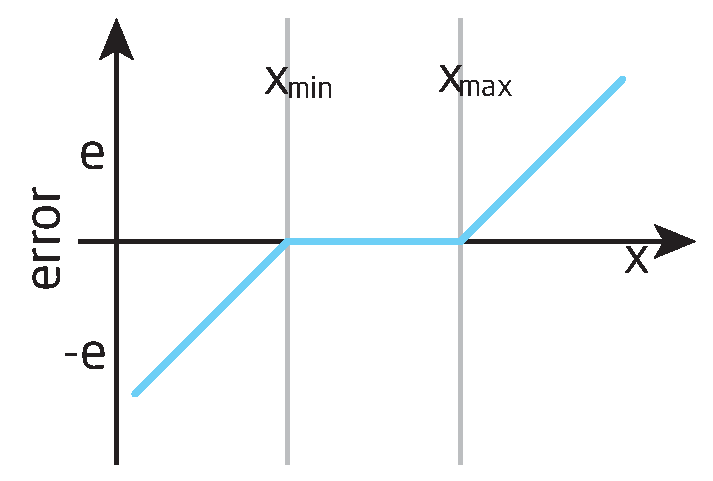
\includegraphics[width=0.5\columnwidth]{SEGAN/band_error2.eps}%
\label{subfig:errorband}}\subfloat[Band service Quality of Service]{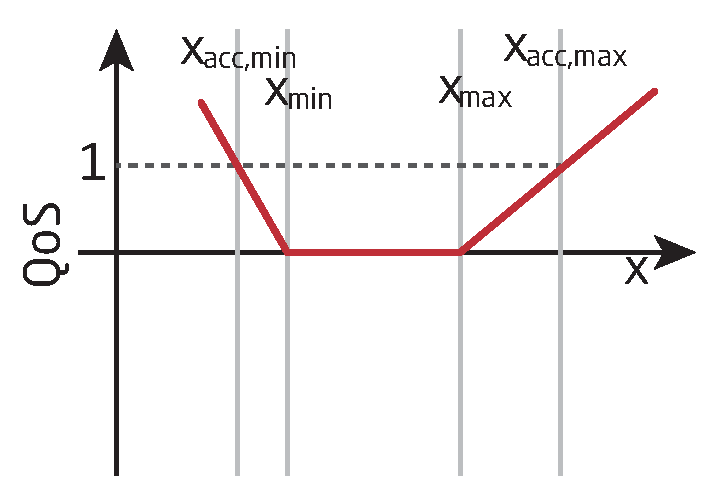
\includegraphics[width=0.5\columnwidth]{SEGAN/band_error3.eps}%
\label{subfig:qosband}}\\
\subfloat[Cap service error]{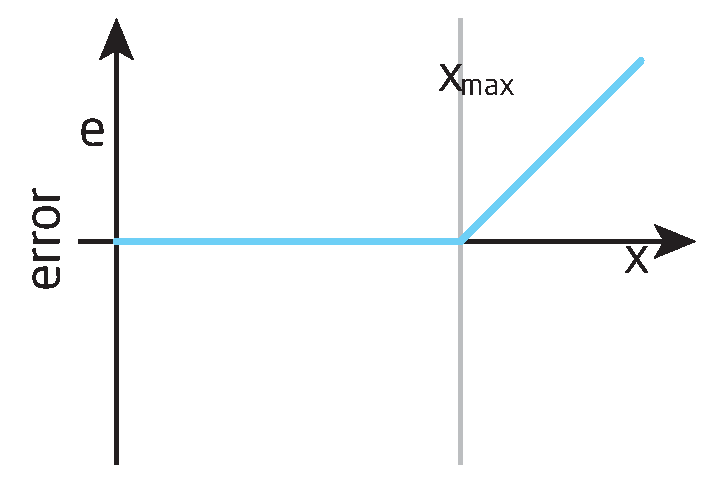
\includegraphics[width=0.5\columnwidth]{SEGAN/cap_error2.eps}%
\label{subfig:errorcap}}
\subfloat[Cap service Quality of Service]{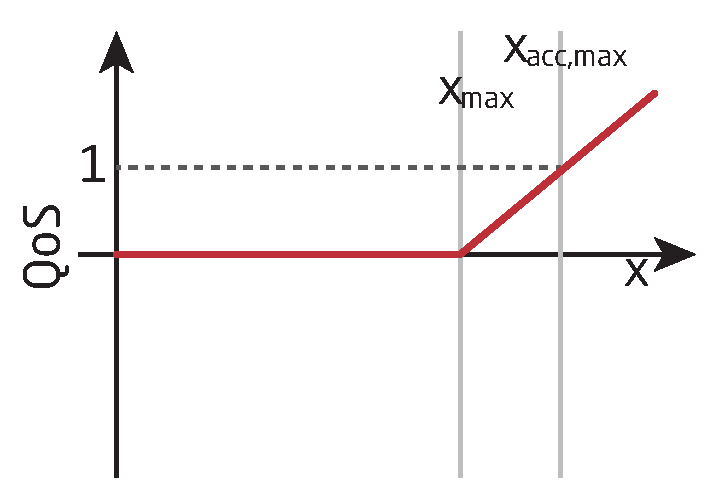
\includegraphics[width=0.5\columnwidth]{SEGAN/cap_error3.eps}%
\label{subfig:qoscap}}
\caption{Error and QoS for the three kinds of services, note that the acceptable band do not need to be symmetric.}
\label{fig:MAINerrorQoS}
\end{figure}

\section{The Aggregator Performance Indices}
\newsection{P}{erformance criteria used for} evaluating controllers usually fall within three categories\fcite{Green}: quality, reliability and energy efficiency. When assessing aggregators, service quality and service reliability define the performance of the aggregator. Four requirements are defined for the performance criteria of aggregators:
\begin{itemize}
	\item[R1] Provide a \emph{quality} measure normalized to the contractual requirements (bounds) of a service. 
	\item[R2] The measure should be normalized with respect to time.
	\item[R3] Provide a \emph{reliability} measure in relation to service non-delivery.
	\item[R4] Each service that the aggregator provides must have a separate, individually verifiable, measure. For example, to evaluate service delivery with respect to ancillary-service delivery, the asset-management quality is irrelevant.
\end{itemize}

To fulfill these requirements two indices are defined:
\begin{itemize}
	\item a service performance assessment index, and
	\item a service verification index.
\end{itemize}

\subsection{Service Performance Assessment index}
The service performance assessment index consists of the weighted average of the normalized root mean square error (RMSE) of the service delivery\footnote{Originally, this index was defined in \cite{bondy2014performance} as the integral square error (ISE) of the service delivery, which was then normalized to a maximum allowable error. This definition does note cope well when the service provision of several services are evaluated at the same time. Therefore, the index was reformulated as the RMSE.}. For evaluation of \emph{K} amount of ancillary services, over discrete time horizon of service delivery \emph{N}, the index is defined:
\begin{align}\label{eq:MAINetaAS}
\eta^{AS} &= \sum^{K}_{i=1} W_i \sqrt{\frac{\sum^{N_i}_{t=0} \left( {QoS^{AS}_{i,t}}^{2} \right)}{N_i}}\\
\sum_{i=1}^K W_i &= 1
\end{align}
where $QoS^{AS}_{i,t}$ is the truncated $QoS \in [0,1]$ of the ancillary serviced delivery. This definition means that $\eta^{AS} \in [0,1]$, where values close to 0 mean a good service delivery, and values close to 1 mean a bad service delivery. It is expected that in most cases $K=1$, but this definition allows for more services being evaluated at the same time.

The index can be similarly defined for \emph{M} amount of asset management services:
\begin{equation}\label{eq:MAINetaAMS}
\eta^{AMS} = \sum^{M}_{i=1} W_i \sqrt{\frac{\sum^{N_i}_{t=0} \left( {QoS^{AMS}_{i,t}}^{2} \right)}{N_i}}.
\end{equation}
It is likely that $M > 1$, e.g. if the aggregator is an EV fleet operator for a single large customer. Finally, if an aggregator desires to evaluate its own overall performance, e.g. as part of an internal reviewing process, it can combine both kinds of service provision in a weighted average:
\begin{equation}
\eta_{tot} = \alpha \eta^{AS} + (1-\alpha) \eta^{AMS}, \quad \alpha \in [0,1]
\end{equation}
where $\alpha$ is the weight ratio  between the two kinds of service.

\subsection{Service Verification Index}
Similar to the service performance assessment index, an index is defined for service verification\footnote{This index can also be interpreted as an index measuring non-delivery.} based upon \emph{QoS} whenever $QoS > 1$. A new measure is introduced:
\begin{equation}
	ND(t) = QoS(t) - 1,\quad \forall QoS(t) > 1, \forall t.
\end{equation}
Using this new measure, the service verification index for \emph{K} amount of ancillary services, over a discrete time horizon of service delivery \emph{N}, is defined as:
\begin{equation}\label{eq:epsilonAS}
\epsilon^{AS} = \sum^{K}_{i=1} W_i \sqrt{\frac{\sum^{N_i}_{t=0} \left( {ND^{AS}_{i,t}}^{2} \right)}{N_i}}
\end{equation}
where $\epsilon^{AS} \in [0,\infty]$. Similar to $\eta$, $\epsilon$ is also normed to time. The service verification for the index can also be defined for asset management services:
\begin{equation}\label{eq:epsilonAMS}
\epsilon^{AMS} = \sum^{M}_{i=1} W_i \sqrt{\frac{\sum^{N_i}_{t=0} \left( {ND^{AMS}_{i,t}}^{2} \right)}{N_i}}.
\end{equation}

For some services, e.g. ancillary services, it is critically important that $QoS(t) \lll 1$, which would mean a requirement of $\epsilon \approx 0}$. In other cases, $\epsilon > 0}$ is tolerable to certain extent. The tolerance limit for $\epsilon$ should be defined in the contract agreements between aggregator and the entity acquiring the services.





\section{Application to Service Verification}

\section{Conclusions on Performance Assessment}
% chapter Service Verification (end)

